\documentclass[a4paper]{jcst}

\usepackage{amssymb}
\setcounter{tocdepth}{3}
\usepackage{graphicx}
%\usepackage{algorithm,algorithmic}
\usepackage{multirow}
\usepackage{bigstrut}
\usepackage{amsmath}
\usepackage{enumitem}

\clubpenalty=10000  %asigna una "penalización" de 10000 al hecho de dejar líneas huérfanas
\widowpenalty=10000 %asigna una "penalización" de 10000 al hecho de dejar líneas viudas.

\usepackage{url}
\newcommand{\keywords}[1]{\par\addvspace\baselineskip
\noindent\keywordname\enspace\ignorespaces#1}

% first the title is needed
\title{Parallelism and Hybridization in Differential Evolution to solve the Flexible Job Shop Scheduling Problem
\\
\large Paralelismo e hibridización en un algoritmo de evolución diferencial para resolver el problema de planificación job shop flexible}

\author[1\orcid{0000-0003-1488-3687}]{Franco Morero}
\author[1\orcid{0000-0001-9767-6194}]{Carlos Bermúdez}
\author[1,2\orcid{0000-0002-3417-8603}]{Carolina Salto}

\affil[1]{LISI - Facultad de Ingenier\'ia, Universidad Nacional de La Pampa, General Pico, Argentina \authorcr
\{bermudezc,saltoc\}@ing.unlpam.edu.ar}
\affil[2]{CONICET, Argentina}

\begin{document}

\maketitle
\begin{abstract}
The Flexible Job Shop Scheduling Problem (FJSSP) is one of the most challenging combinatorial optimization problems, with practical applicability in a real production environment. In this work, we propose a simple Differential Evolution (DE) algorithm to tackle this problem. To represent a FJSSP solution, a real value representation is adopted, which requires a very simple conversion mechanism to obtain a feasible schedule. Consequently, the DE algorithm still works on the continuous domain to explore the problem search space of the discrete FJSSP. Moreover, to enhance the local search ability and to balance the exploration and exploitation capabilities, a simple local search algorithm is embedded in the DE framework. Also, the parallelism of the DE operations is included to improve the efficiency of the whole algorithm. Experimental results confirm the significant improvement achieved by integrating the modifications introduced in this study. Additionally, test results show that our algorithm is competitive when compared with most existing approaches for FJSSP.


\end{abstract}

\keywords{differential evolution, flexible job shop scheduling, parallelism}

\renewcommand{\abstractname}{Resumen}
\begin{abstract}
El problema de planificación \textit{job shop} flexible (FJSSP, en inglés) es uno de los problemas de optimización más desafiantes, con aplicabilidad práctica en ambientes de producción real. En este trabajo, se propone un algoritmo de evolución diferencial (DE, en inglés) simple para resolver el problema en cuestión. Para representar una solución al FJSSP, se adopta una representación de vectores reales, la cual requiere un mecanismo de conversión muy simple para obtener una planifación factible. Consecuentemente, el algoritmo DE continúa trabajando en el dominio continuo para explorar el espacio de búsqueda del problema que es de caracter discreto. Además, para mejorar la habilidad de búsqueda local y lograr un equilibrio entre la exploración y explotación, se incorpora un algoritmo de búsqueda local simple. También, se incluye paralelismo a las operaciones del DE para mejorar la eficiencia del algoritmo. Los resultados obtenidos confirman que el rendimiento del DE mejora en forma significativa al incorporar las propuestas incluidas en este estudio.
Además, los resultados de las pruebas muestran que nuestro algoritmo es competitivo en comparación con la mayoría de los existentes.
\end{abstract}

\palabrasclaves{evolución diferencial, paralelismo, planificación de trabajos}

\input{sections/introducción}

\section{The Flexible Job Shop Scheduling Problem} \label{sec:FJSSP}
\vspace{-0.4cm}

FJSSP is an extension of the classic JSSP where a set of machines, not necessarily identical, can process an operation. Consequently, a set of available machines is provided for each operation. The goal is to decide on which machine each operation will be assigned and in what order the operations will be sequenced on each machine so that the makespan is minimized.

FJSSP can be formally described as follows. A set $J = \{J_1, J_2,\ldots, J_n\}$ of independent jobs and a set $U = \{M_1,M_2, \ldots, M_m\}$ of machines are given. A job $J_i$ is broken down by a sequence of $O_{i1},O_{i2}, \ldots, O_{in_i}$ operations to be performed one after the other according to the given sequence. Each operation $O_{ij}$ can be executed on any among a subset $U_{ij} \subseteq U$ of compatible machines. For this reason, the FJSSP can be classified into two categories, partial (P-FJSSP) and total (T-FJSSP)  \cite{kacem2002}. We have partial flexibility whether exists a proper subset $U_{ij} \subset U$, for at least one operation $O_{ij}$, while we have $U_{ij} =U$ for each operation $O_{ij}$ in the case of total flexibility. The processing time of each operation is machine-dependent. 
Pre-emption is not allowed, i.e., each operation must be completed without interruption once started. Furthermore, the machines cannot perform more than one operation at a time. All jobs and machines are available at time 0.

The problem is to assign each operation to an appropriate machine (routing problem),  and  sequence the operations on the machines (sequencing problem) to minimize the makespan ($C_{max}$). This measure is the time needed to complete all the jobs, which is defined as $C_{max} = max_i\{C_i\}$, where $C_i$ is the completion time of the job $J_i$.  Table~\ref{tab:proccesingTime} shows an instance of FJSSP with 3 jobs, 4 machines and 8 operations. The rows and columns correspond to machines and operations, respectively, and the entries of the table are the processing times. 

\begin{table}[tb]
\scriptsize
   \centering
   \caption{Instance Example for FJSSP}
   \label{tab:proccesingTime}%
\begin{tabular}{c|ccc|ccc|cc}
\hline
\multicolumn{1}{l|}{} & \multicolumn{3}{c}{$J_1$} & \multicolumn{3}{c}{$J_2$} & \multicolumn{2}{c}{$J_3$} \\
\hline
\multicolumn{1}{l|}{} & $O_{11}$    & $O_{12}$   & $O_{13}$   & $O_{21}$    & $O_{22}$   & $O_{23}$   & $O_{31}$        & $O_{32}$       \\
\hline
$M_1$                   & -      & 4     & 9     & 2      & 4     & 9     & 8          & 3         \\
$M_2$                   & 6      & 8     & 5     & -      & 6     & -     & 6          & 5         \\
$M_3$                   & 5      & 5     & -     & 1      & 8     & 2     & -          & 8         \\
$M_4$                   & -      & 6     & 7     & 3      & 4     & 2     & 5          & 3        \\
\hline
\end{tabular}
\end{table}
 %problem description

\section{Differential Evolution Algorithm: Background}
\label{sec:DE}
\vspace{-0.4cm}
The DE algorithm was proposed by Storn and Price~\cite{Storn1997} to solve optimization problems with real-valued parameters. DE is a stochastic, population-based  optimization method. Despite having a very simple algorithmic structure, DE has demonstrated a high level of performance when solving a wide variety of very complex problems~\cite{Price:2005}. The optimal or near-optimal solution is obtained by an iterative process which is applied to a set of solutions (population) to achieve a new one. At each step of the process, new solutions arise as a result of perturbations to the current solutions, caused by mutation and recombination operators. %The general structure of the DEA shares similar features with other evolutionary algorithms, such as genetic algorithm (GA)~\cite{holland75}. DE algorithm is different in handling distance and direction information to move the population at the current generation toward the next generation, in virtue of a constructive cooperation between individuals.

The algorithmic framework of DE is described in Algorithm~\ref{alg:algoritmoDE}. The first step (Line 1) consists in the initialization of the population $P^0$ of $N_P$ target vectors of \textit{D} real values ($x_i = (x_{i,1}, x_{i,2}, . . . , x_{i,D}) \in \mathbb{R}^{D}  (1 \leq i \leq N_P)$). Each component $x_{i,j} \in \mathbb{R} (1 \leq j \leq D)$ represents a variable or a parameter of the optimization problem. Usually, each $x_{i,j}$ is bounded to a value in the range $[li_j, ls_j]$, where $li_j$, $ls_j \in \mathbb{R}$ are the lower and upper bound, respectively. The $N_P$ target vectors are initialized randomly by applying Equation~\ref{eqDE:Init}:
\vspace{-0.2cm}
\begin{equation}\label{eqDE:Init}
x_{i,j} = li_{j} + U(0, 1) \times (ls_j - li_j)
\end{equation}
%\vspace{-0.1cm}
\noindent where $U(0, 1)$ is a random number with uniform distribution in the range $[0, 1]$. 

\begin{algorithm}[tb]
\scriptsize
    \caption{Differential Evolution Algorithm (DE)} \label{alg:algoritmoDE}
    \begin{algorithmic} [1]
    \Require {$F, Cr, N_p$} 
    \Ensure {$x_{best}$} 
        \State initialize($P^0$,$N_p$) 
        \State $g \leftarrow 0$
        \While {not meet stop criterion}
            \For {each vector $x_{i}^g$ from $P^g$}
                \State $v_{i}^g \leftarrow $ mutate($x_{i}^g, P^g, F$) 
                \State $u_{i}^g \leftarrow $ recombinate($x_{i}^g, v_{i}^g, Cr$)
                \State $x_{i}^g \leftarrow $ select($x_{i}^g, u_{i}^g$)
                \State add($P^{g+1}, x_{i}^{g+1}$) 
            \EndFor
            \State $g \leftarrow g+1$ 
        \EndWhile
        \State$x_{best} \leftarrow $best\_solution($P^{g}$)
    \end{algorithmic}
\end{algorithm}


%After the initialization step, an iterative process begins, which consists in the application of mutation (Line 5 of Algorithm~\ref{alg:algoritmoDE}), recombination (Line 6), and selection (Line 7) operations until an stop criterion is reached. 

After the initialization step, an iterative process begins. The mutation operation (Line 5 of Algorithm~\ref{alg:algoritmoDE}) obtains a donor vector $v_i^g = (v_{i,1}, v_{i,2}, . . . , v_{i,D})$ for each target vector $x_i^g$ from the current population $P^g$ ($0 \leq g \leq max_{gen}$) following Equation~\ref{eqDE:mutation}. To obtain $v_i^g$, a base vector $x_{r0}^g$ and other two vectors $x_{r1}^g$ y $x_{r2}^g$ are randomly selected from $P^g$, with $r0, r1$ and $r2$ chosen from the set $\{1,2,...,N_P\}$ and all of them are mutually exclusive. The $F \in [0 . . . 1)$ factor, known as scale factor, controls the rate at which the population evolves, in order to avoid their stagnation during the search process. The mutation operator is important to the DE's behaviour because it focuses the search on the most promising areas of the solution space. 
\vspace{-0.1cm}
\begin{equation}\label{eqDE:mutation} 
v_i^g = x_{r0}^g + F \times (x_{r1}^g - x_{r2}^g)
\end{equation}
%\vspace{-0.4cm}
The donor vector is modified by the recombination operator (Line 6), with the aim of increasing the population diversity. This operator creates a trial vector $u_i^g$ through mixing components of the donor vector $v_i^g$ and the target vector $x_i^g$. The most frequently referred crossover operator is the binomial crossover, which is shown in Equation~\ref{eqDE:recombination}:
\vspace{-0.4cm}
\begin{equation} \label{eqDE:recombination}
u_{i,j}^g = \left\lbrace
\begin{array}{ll}
v_{i,j}^g & \textup{si } r_j < Cr \vee j = j_r\\
x_{i,j}^g & \textup{otherwise} 
\end{array}
\right.
\end{equation}
%\vspace{-0.4cm}
\noindent where $r_j=U(0, 1)$ is a random value, $j_r$ is also a random value in the set \{1, 2, ...,$D$\}, and finally $Cr$ is a parameter known as recombination probability, which controls the fraction of parameter values that are copied from the donor.

The last step %in the DE's iterative process 
is the selection operation (Line 7). The trial vector $u_{i}^g$ competes against the target vector $x_{i}^g$ regarding their objective values (obtained applying the objective function to each vector). The best vector is selected to be part of the population $P^{g+1}$ of the next generation%(see the Equation~\ref{eqDE:selection})
. Clearly, this competition %between parents and children 
creates a new population with a performance equal or superior to the current one (Line 8). Consequently, DE is an elitist evolutionary algorithm. 

%\begin{equation} ~\label{eqDE:selection}
%x_{i}^{g+1} = \left\lbrace
%\begin{array}{ll}
%u_{i}^g & \textup{if } f(u_{i}^g) \textup{ \textit{ is equal or best than} } f(x_{i}^g)\\
%x_{i}^g & \textup{otherwise} 
%\end{array}
%\right.
%\end{equation}

The stopping criteria can be set to a preset maximum number of iterations ($max_{gen}$) or some other problem-dependent criterion. Whichever the criteria to be set, the choice has a direct influence on the best solution $x_{best}$ obtained by the algorithm (Line 12). 

DE performance mainly depends on three parameters: scaling factor of the difference vector ($F$), crossover control parameter ($Cr$) and population size ($N_P$). Some guidelines are available to choose the control parameters~\cite{Price:2005}. In this work, $N_P$ and $F$ are chosen  based  on  previous  knowledge  and  keep  it  constant during all runs. % The factor $F$ usually takes a value that ranges from 0.4 to 1.0~\cite{Gamperle02aparameter}. 
On the other hand, a good value for $Cr$ is 0.1 however, to speed up convergence a greater value can be used. %DE description

\section{Our proposal: Hybrid DE for the FJSSP}
\label{sec:HDE}
\vspace{-0.2cm}
In this section, our proposal to solve the  FJSSP is detailed. In order to apply the DE algorithm, it is crucial to design a suitable encoding scheme that maps the floating point vectors to the feasible solution for the FJSSP (see Section~\ref{subsec:rep}). Moreover, our proposal is enhanced by a simple local search (Section~\ref{subsec:HDE}). Finally, a parallel version of our proposal is introduced (Section~\ref{subsec:parallelHDE}).


\subsection{Representation}  \label{subsec:rep}
\vspace{-0.25cm}
In this work, the DE algorithm still manipulates real-valued vector in order to maintain the simplicity and properties of the DE in their natural configuration. Consequently, the schedule is generated following the random keys encoding scheme~\cite{Bean1994RepRandomKeys}. This representation deals with real point vectors, where these points are used as sort keys to decode the solution. For an $n$-job $m$-machine scheduling problem, each vector's position (a random key) consists of a floating number in U(-1,1) which can be translated to an unique list of ordered operations, after a descending order of the random keys. These steps always obtain a feasible schedule from a real-valued vector. The schedule is a permutation with repetitions~\cite{bierwirth1995}. See Figure~\ref{fig:decodificacion} for an example considering the instance shown in Table~\ref{tab:proccesingTime}. Given the vector $x_i^g$=[0.6,-0.5,0.4,-0.3,-0.1,0.9,-0.7,0.2], it is converted to a schedule $[2, 1, 1, 3, 2, 2, 1, 3]$, which is a permutation of the set of operations that represents a tentative ordering to schedule them, each one being represented by its job number. This valid schedule corresponds to the operation sequence $O_{21}$, $O_{11}$, $O_{12}$, $O_{31}$, $O_{22}$, $O_{23}$, $O_{13}$, and $O_{32}$. 

In order to evaluate $x_i^g$, the objective value is the makespan ($C_{max}$). To compute it, each operation $O_{ij}$ in $x_i^g$ is assigned to a feasible machine $M_k$ in $U_{ij}$ with the shortest completion time, and then the load of $M_k$ must be updated. The initial solution is generated by a random procedure (Equation 1), mainly because high performing construction heuristics for the FJSSP are unknown.
%
%The decoding procedure is explained in Algorithm~\ref{alg:algoritmoDecodificacion} and is applied before the evaluation of an vector begins. An illustrative example is shown in FigureXX.
%
%En la figura \ref{fig:decodificacion} se puede ver un ejemplo de este procedimiento para una instancia del problema FJSSP con 3 trabajos, 4 máquinas y 8 operaciones mostrada en la tabla
%
\begin{figure}[tb]
    \centering
    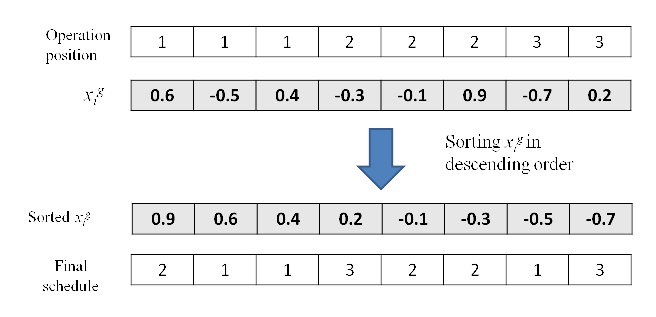
\includegraphics[width=0.55\textwidth]{./figures/deco.eps}
    \caption{Example of the decoding process used by the DE to solve the FJSSP.}
    \label{fig:decodificacion}
    \vspace{-0.4cm}
\end{figure}
%
\subsection{DE and Local Search Method} \label{subsec:HDE}
\vspace{-0.25cm}
DE is enhanced with a local search technique, yielding a hybrid DE (HDE) for exploration and exploitation among the solutions to obtain a near optimal solution. In this work, a simple interchange mechanism is implemented in which two positions of the target vector are randomly selected  and interchanged. If there is an improvement in the objective function the swap is accepted, otherwise, it is not considered. %The pseudo-code of local search procedure is given in Figure~\ref{alg:algoritmoLS}. 
This local search procedure is applied to the target vectors $x_{i}$ of the next population (just before Line 11 of Algorithm~\ref{alg:algoritmoDE}) but not to the trial vector $u_{i}$, which is beneficial to avoid both cycling search and getting trapped in a local optimum. Moreover, the frequency of the local search is controlled by the probability $p_{LS}$. Another important characteristic of this local search procedure is that it does not need a backward conversion because it is applied over the real-valued vector.
%
%
%Con el fin de mejorar la eficiencia de DE, se incorporó al algoritmo un procedimiento de busqueda local, que actua sobre la población justo antes de la línea 10 del algoritmo \ref{alg:algoritmoDE}. En el algoritmo \ref{alg:algoritmoLS} se puede ver un pseudocodigo del proceso realizado, el cual consiste en iterar sobre todos los individuos de la población, obtener un número aleatorio y si es menor a una probabilidad de aplicar busqueda local realizar las siguientes acciones: seleccionar 2 indices aleatorios en el individuo $x_{i}$, intercambiar entre ellos obteniendo un nuevo vector de prueba $u_{i}$, y si al evaluar $u_{i}$ obtenemos una solución igual o mejor que $x_{i}$, seleccionar $u_{i}$ como nuevo individuo de nuestra población.
%
%\begin{algorithm} [H]
%    \caption{Local Search Procedure} \label{alg:algoritmoLS} 
%    \begin{algorithmic} [1]
%        \For {each $x_{i}^g$ from $P^{g}$}
%            \If {$random() < PBL$} %\Comment PBL: probabilidad de busqueda local
%                \State $j$ , $k \leftarrow $ random(1,$D$)
%                \State $u_{i} \leftarrow $ swap($x_{i}$, $j$,$k$)
%                \If {$f(u_{i}) \leq  f(x_{i})$} \Comment{for a minimization problem}
%                    \State $x_{i} \leftarrow u_{i}$
%                \EndIf
%            \EndIf
%        \EndFor
%    \end{algorithmic}
%\end{algorithm}

\subsection{DE and Parallelism} \label{subsec:parallelHDE}
\vspace{-0.2cm}
In terms of designing parallel metaheuristics, the DE can be paralleled in different ways~\cite{Talbi}. %For instance, their population-based characteristics allow evaluating in a parallel way the fitness value of each individual, giving rise a global or master-slave model. In this same line, each iteration of a metaheuristic can be parallelized. In this two cases, the behaviour of the metaheuristic is not altered. Parallelism can also be exploited to perform the genetic operators in a semi-isolated manner, resulting in the island model. Finally, the previous strategies can be combined, giving rise to the cellular model~\cite{albaPEA2006}. This last two models alter the behavior of the metaheuristic and enable the improvement of the quality of solutions.
In this work, the aim of the parallelization is not to change the behaviour of the metaheuristic but to speed up the search. For that purposes, we focus on the parallelization of each iteration of the DE~\cite{albaPEA2006}. The population of individuals is decomposed and handled in parallel, using the well-known global parallelization model. A principal process performs the selection operations and the replacement, which are generally sequential. The rest processes (workers) perform the mutation, recombination, and the evaluation of the solutions in parallel. Consequently, this model maintains the sequence of the original algorithm, and hence the behavior of the metaheuristic is not altered. 








%Actuando sobre la eficiencia del algoritmo, con el fin de mejorar la velocidad del mismo, se optó por un esquema de ejecución en paralelo. Teniendo en cuenta que a cada individuo se lo trata por separado en el proceso de evolución, se cosideró realizar estas ejecuciones en paralelo, tomando cantidades iguales de individuos de la poblacion y asignando cada parte a unidades de procesamiento diferentes. La misma idea se tomo para mejorar la eficiencia en la búsqueda local, otorgando grandes ventajas en cuanto a velocidad y aprovechamiento de recursos.

%\subsection{Implementación de \textit{DE} híbrido para \textit{FJSSP}}
%El algoritmo \ref{alg:algoritmoDEhibrido} presenta el pseudocodigo del algoritmo de \textit{DE} hibrido para \textit{FJSSP}. Como se puede observar el esquema general es el mismo que el presentado anteriormente, con la inclusión del proceso de búsqueda local. Además, se agrega como entrada la probabilidad de aplicar busqueda local ($PBL$).

%\begin{algorithm} [H]
%    \caption{Pseudocodigo de la Evolucion Diferencial (DE)} \label{alg:algoritmoDEhibrido}
%    \begin{algorithmic} [1]
%    \Require {$F, Cr, N_p, PBL$} 
%    \Ensure {$x_{best}$} 
%        \State inicializar($P$,$N_p$) 
%        \State $g \leftarrow 0$
%        \While {no se alcance la condición de fin}
%            \For {cada vector $x_{i}^g$ de $P^g$}
%                \State $v_{i}^g \leftarrow $ mutacion($x_{i}^g, P^g, F$) 
%                \State $u_{i}^g \leftarrow $ recombinacion($x_{i}^g, v_{i}^g, Cr$)
%                \State $x_{i}^g \leftarrow $ seleccion($x_{i}^g, u_{i}^g$)
%                \State agregar($P^{g+1}, x_{i}^{g+1}$) 
%            \EndFor
%            \State busqueda-local($P^g$, $PBL$)
%            \State $g \leftarrow g+1$ 
%        \EndWhile
%        \State$x_{best} \leftarrow $mejor-solucion($P^{g}$)
%
%    \end{algorithmic}
%\end{algorithm}



 %DE description

\section{Experimental Design} \label{sec:experDesig}

In this section, we describe the experimental design followed in this approach. We have selected a wide range of FJSSP instances used in the literature taking into account their complexity, which is given by the number of jobs and machines, and the wide variation of flexibility in the number of available machines per operation. In this sense, we considered the data set proposed by Brandimarte~\cite{brandimarte1993} as a representative one. The number of jobs ranges from 10 to 20, the number of machines belongs to the set \{4,15\} and the number of operations for each job varies from 5 to 15. Consequently, the total number of operations ranges from 55 to 240. The flexibility is between 1.43 and 4.10.

Concerning the methodology followed to analyze the results, first, we studied the behavior of these algorithms with different $F$ and $Cr$ values, considering the best $C_{max}$ found and the number of iterations to reach them for each instance. This analysis allows us to determine the best values for the control parameters. Secondly, we determined the impact of incorporating a local search procedure at different rates of $p_{LS}$. For this purpose, we take into account the best $C_{max}$ found, and the number of iterations to reach the best solution for each instance. Finally, we study DE's behaviour including parallelism regarding the execution time of each approach. The analyses are principally validated by the data in the tables and figures shown in the experimental research section.

The parametric configuration considered for DE's experimentation is the following. The population size $N_P$ is set to 50. The $F$ factor and the $Cr$ probability are tested with three different values (0.1, 0.5, and 0.9). For the remaining parameter, $p_{LS}$, three values are also analysed (0.1, 0.5 and 0.7). Table~\ref{tab:parameteres} shows a summary of the parameters.

\begin{table}[tb]
\scriptsize
\centering
\caption{Parameter Values}
\begin{tabular}{cc}
\hline
\multicolumn{1}{c}{Parameter} & \multicolumn{1}{c}{Values} \\ 
\hline
NP                              & 50                          \\
F                               & 0.5, 0,7, and 0,9           \\
Cr                              & 0.1 and 0.9                 \\
$p_{LS}$                          & 0.5, 0,7, and 0,9          \\
\hline
\end{tabular}
\label{tab:parameteres}
\end{table}
%
\begin{table*}[!tb]
    \scriptsize
  \centering
  \caption{Best values of $ C_{max} $ found by the DE algorithm with different $F$ and $Cr$ values for all FJSSP instances}
    \begin{tabular}{rrccccccccc|}
    \hline
\multicolumn{1}{|c|}{} & \multicolumn{1}{c|}{} & \multicolumn{3}{c|}{\textbf{F=0.1}} & 
\multicolumn{3}{c|}{\textbf{F=0.5}} & 
\multicolumn{3}{c|}{\textbf{F=0.9}}  \bigstrut\\
    \cline{3-11}
    \multicolumn{1}{|c|}{{\textbf{Inst.}}} & \multicolumn{1}{c|}{{\textbf{Opt.}}} & \multicolumn{1}{c|}{\textbf{Cr=0.1}} & \multicolumn{1}{c|}{\textbf{Cr=0.5}} & \multicolumn{1}{c|}{\textbf{Cr=0.9}} & \multicolumn{1}{c|}{\textbf{Cr=0.1}} & \multicolumn{1}{c|}{\textbf{Cr=0.5}} & \multicolumn{1}{c|}{\textbf{Cr=0.9}} & \multicolumn{1}{c|}{\textbf{Cr=0.1}} & \multicolumn{1}{c|}{\textbf{Cr=0.5}} & \multicolumn{1}{c|}{\textbf{Cr=0.9}} \bigstrut\\
    \hline
    \multicolumn{1}{|c|}{Mk01} & \multicolumn{1}{c|}{40} & \multicolumn{1}{c|}{\textbf{40}} & \multicolumn{1}{c|}{\textbf{40}} & \multicolumn{1}{c|}{\textbf{40}} & \multicolumn{1}{c|}{\textbf{40}} & \multicolumn{1}{c|}{\textbf{40}} & \multicolumn{1}{c|}{\textbf{40}} & \multicolumn{1}{c|}{\textbf{40}} & \multicolumn{1}{c|}{\textbf{40}} & \textbf{40} \bigstrut\\
    %\hline
    \multicolumn{1}{|c|}{Mk02} & \multicolumn{1}{c|}{26} & \multicolumn{1}{c|}{\textbf{26}} & \multicolumn{1}{c|}{27} & \multicolumn{1}{c|}{27} & \multicolumn{1}{c|}{\textbf{26}} & \multicolumn{1}{c|}{27} & \multicolumn{1}{c|}{\textbf{26}} & \multicolumn{1}{c|}{27} & \multicolumn{1}{c|}{27} & 27 \bigstrut\\
    %\hline
    \multicolumn{1}{|c|}{Mk03} & \multicolumn{1}{c|}{204} & \multicolumn{1}{c|}{\textbf{204}} & \multicolumn{1}{c|}{\textbf{204}} & \multicolumn{1}{c|}{\textbf{204}} & \multicolumn{1}{c|}{\textbf{204}} & \multicolumn{1}{c|}{\textbf{204}} & \multicolumn{1}{c|}{\textbf{204}} & \multicolumn{1}{c|}{\textbf{204}} & \multicolumn{1}{c|}{\textbf{204}} & \textbf{204} \bigstrut\\
    %\hline
    \multicolumn{1}{|c|}{Mk04} & \multicolumn{1}{c|}{60} & \multicolumn{1}{c|}{\textbf{60}} & \multicolumn{1}{c|}{\textbf{60}} & \multicolumn{1}{c|}{65} & \multicolumn{1}{c|}{61} & \multicolumn{1}{c|}{\textbf{60}} & \multicolumn{1}{c|}{\textbf{60}} & \multicolumn{1}{c|}{62} & \multicolumn{1}{c|}{63} & 62 \bigstrut\\
    %\hline
    \multicolumn{1}{|c|}{Mk05} & \multicolumn{1}{c|}{172} & \multicolumn{1}{c|}{175} & \multicolumn{1}{c|}{173} & \multicolumn{1}{c|}{173} & \multicolumn{1}{c|}{175} & \multicolumn{1}{c|}{179} & \multicolumn{1}{c|}{173} & \multicolumn{1}{c|}{175} & \multicolumn{1}{c|}{179} & 173 \bigstrut\\
    %\hline
    \multicolumn{1}{|c|}{Mk06} & \multicolumn{1}{c|}{58} & \multicolumn{1}{c|}{65} & \multicolumn{1}{c|}{59} & \multicolumn{1}{c|}{63} & \multicolumn{1}{c|}{66} & \multicolumn{1}{c|}{69} & \multicolumn{1}{c|}{59} & \multicolumn{1}{c|}{67} & \multicolumn{1}{c|}{70} & 61 \bigstrut\\
    %\hline
    \multicolumn{1}{|c|}{Mk07} & \multicolumn{1}{c|}{139} & \multicolumn{1}{c|}{143} & \multicolumn{1}{c|}{140} & \multicolumn{1}{c|}{142} & \multicolumn{1}{c|}{143} & \multicolumn{1}{c|}{148} & \multicolumn{1}{c|}{140} & \multicolumn{1}{c|}{144} & \multicolumn{1}{c|}{146} & 140 \bigstrut\\
    %\hline
    \multicolumn{1}{|c|}{Mk08} & \multicolumn{1}{c|}{523} & \multicolumn{1}{c|}{\textbf{523}} & \multicolumn{1}{c|}{\textbf{523}} & \multicolumn{1}{c|}{\textbf{523}} & \multicolumn{1}{c|}{\textbf{523}} & \multicolumn{1}{c|}{\textbf{523}} & \multicolumn{1}{c|}{\textbf{523}} & \multicolumn{1}{c|}{\textbf{523}} & \multicolumn{1}{c|}{\textbf{523}} & \textbf{523} \bigstrut\\
    %\hline
    \multicolumn{1}{|c|}{Mk09} & \multicolumn{1}{c|}{307} & \multicolumn{1}{c|}{318} & \multicolumn{1}{c|}{\textbf{307}} & \multicolumn{1}{c|}{310} & \multicolumn{1}{c|}{321} & \multicolumn{1}{c|}{333} & \multicolumn{1}{c|}{\textbf{307}} & \multicolumn{1}{c|}{321} & \multicolumn{1}{c|}{338} & \textbf{307} \bigstrut\\
    %\hline
    \multicolumn{1}{|c|}{Mk10} & \multicolumn{1}{c|}{197} & \multicolumn{1}{c|}{237} & \multicolumn{1}{c|}{210} & \multicolumn{1}{c|}{221} & \multicolumn{1}{c|}{238} & \multicolumn{1}{c|}{245} & \multicolumn{1}{c|}{206} & \multicolumn{1}{c|}{240} & \multicolumn{1}{c|}{246} & 215 \bigstrut\\
    \hline
      \multicolumn{2}{c|}{}   & 5/10 & 5/10 & 3/10 & 4/10 & 4/10 & \textbf{6/10} & 3/10 & 3/10 & 4/10 \bigstrut\\
    \cline{3-11}
    \end{tabular}%
   \label{tab:resultDE}
\end{table*}%

Because of the stochastic nature of the algorithms, we performed 30 independent runs of each test to gather meaningful experimental data and apply statistical confidence metrics to validate our conclusions. Before performing the statistical tests, we first checked whether the data followed a normal distribution by applying the Shapiro-Wilks test. Where the data was distributed normally, we later applied an ANOVA test. Otherwise, we used the Kruskal-Wallis (KW) test to assess whether or not there were meaningful differences between the compared algorithms with a confidence level of 99\%.

The considered algorithms were programmed in C++. Consequently, their runtimes are directly comparable. All algorithms were compiled on the same computer with the same compilation flags, and run on homogeneous hardware. All are positive attributes of a comparison. The experimentation is carried out on a cluster of 4 INTEL I7 3770K quad-core processors, 8 GB RAM, and the Slackware Linux with a 2.6.27 kernel version. To implement the parallel version of DE, a portable programming interface for shared memory parallel computers such us OpenMP~\cite{openMP} is used.



\section{Experimental Results}

In this subsection, we analyze the result quality considering the $C_{max}$ values obtained from the DE algorithm to solve FJSSP, described in previous sections. First, the influence of $Cr$ and $F$ parameters in the DE performance to solve FJSSP is studied (Section~\ref{subsec:Parameters}). Next, the incorporation of the local search process to the DE using different $p_{LS}$ values is analyzed in Section~\ref{subsec:resparallelDELS}. Finally, the parallel implementation of $DE_{LS}$ is considered in Section~\ref{subsec:resparallelDELS}. 

\subsection{Influence of DE Parameters} \label{subsec:Parameters}

The first analysis focuses on the effect of using different combinations of $F$ and $Cr$ values on the performance of DE to solve FJSSP. In particular, both parameters take values in \{0.1, 0.5, 0.9\}, from low to high values. For this purpose, we analyze the result quality taking into account the best $C_{max}$ values obtained for the simple DE algorithm when solving FJSSP instances, and also the number of evaluations needed to reach their best values.

Table~\ref{tab:resultDE} shows the best $C_{max}$ values obtained for the DE algorithm using the different combinations of $F$ and $Cr$ values for each FJSSP instance. Column 2 presents the best-known value of $C_{max}$ (optimal) for each instance. The last row displays the ratio of the number of instances that an algorithm can find its optimum to the total number of instances. 

The DE finds the optimum in 3 instances (MK01, MK03, and MK08) independently from the combinations of $F$ and $Cr$ values considered. The highest value of $F$ offers the less chance of finding the best solutions for the DE regardless of the $Cr$ value used. This combination presents the lowest number of optimal values for the different instances (no more than 4 of the 10 instances). The DE algorithm with the combination of $F=0.5$ and $Cr=0.9$ finds more times the optimal $C_{max}$ value than the others (in 6 of the 10 instances).

An important metric is the relative error or gap of the different best $C_{max}$ values obtained for each DE regarding the optimum of each instance. This metric allows us to normalized the data of the different instances and, in this way, we focus the attention on how different combinations of $F$ and $Cr$ values affect the performance of the DE to solve FJSSP. On the one hand, KW statistical test indicates that there are significant statistical differences between the DE combinations (\textit{p}-value$=2.2e-16$ is lower to the significance level $\alpha = 0.01$). On the other hand, the gap distribution for each combination (see Figure~\ref{fig:DEboxplot}) suggests that the DE algorithm with $F=0.5$ and $Cr=0.9$ presents the lowest median relative error, and also, its box is comparatively short suggesting that overall gap values have a high level of similarity with each other. These observations indicate a superiority of the combination over the other possible ones.  

\begin{figure}[!tb]
    \centering
    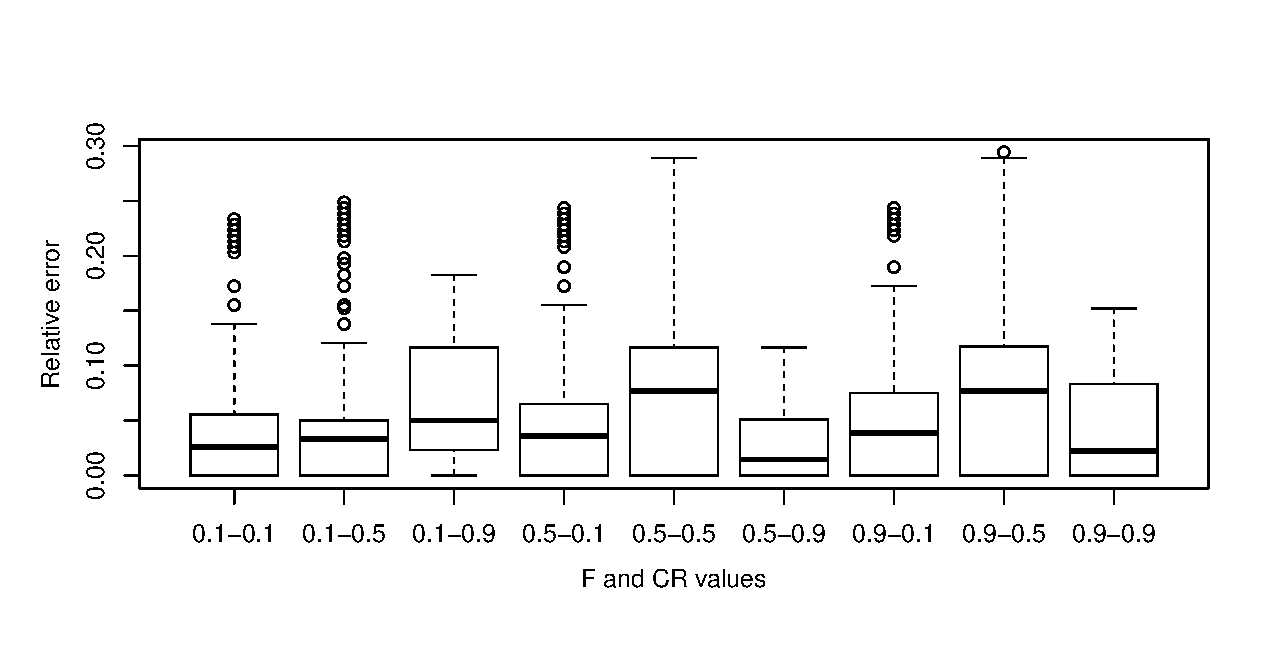
\includegraphics[width=\linewidth]{./figures/Boxplot-DE.eps}
    \caption{Relative error of the DE algorithm for different combinations of $F$ and $Cr$ values.}
    \label{fig:DEboxplot}
\end{figure}
%
\begin{figure*}[htb]
    \centering
    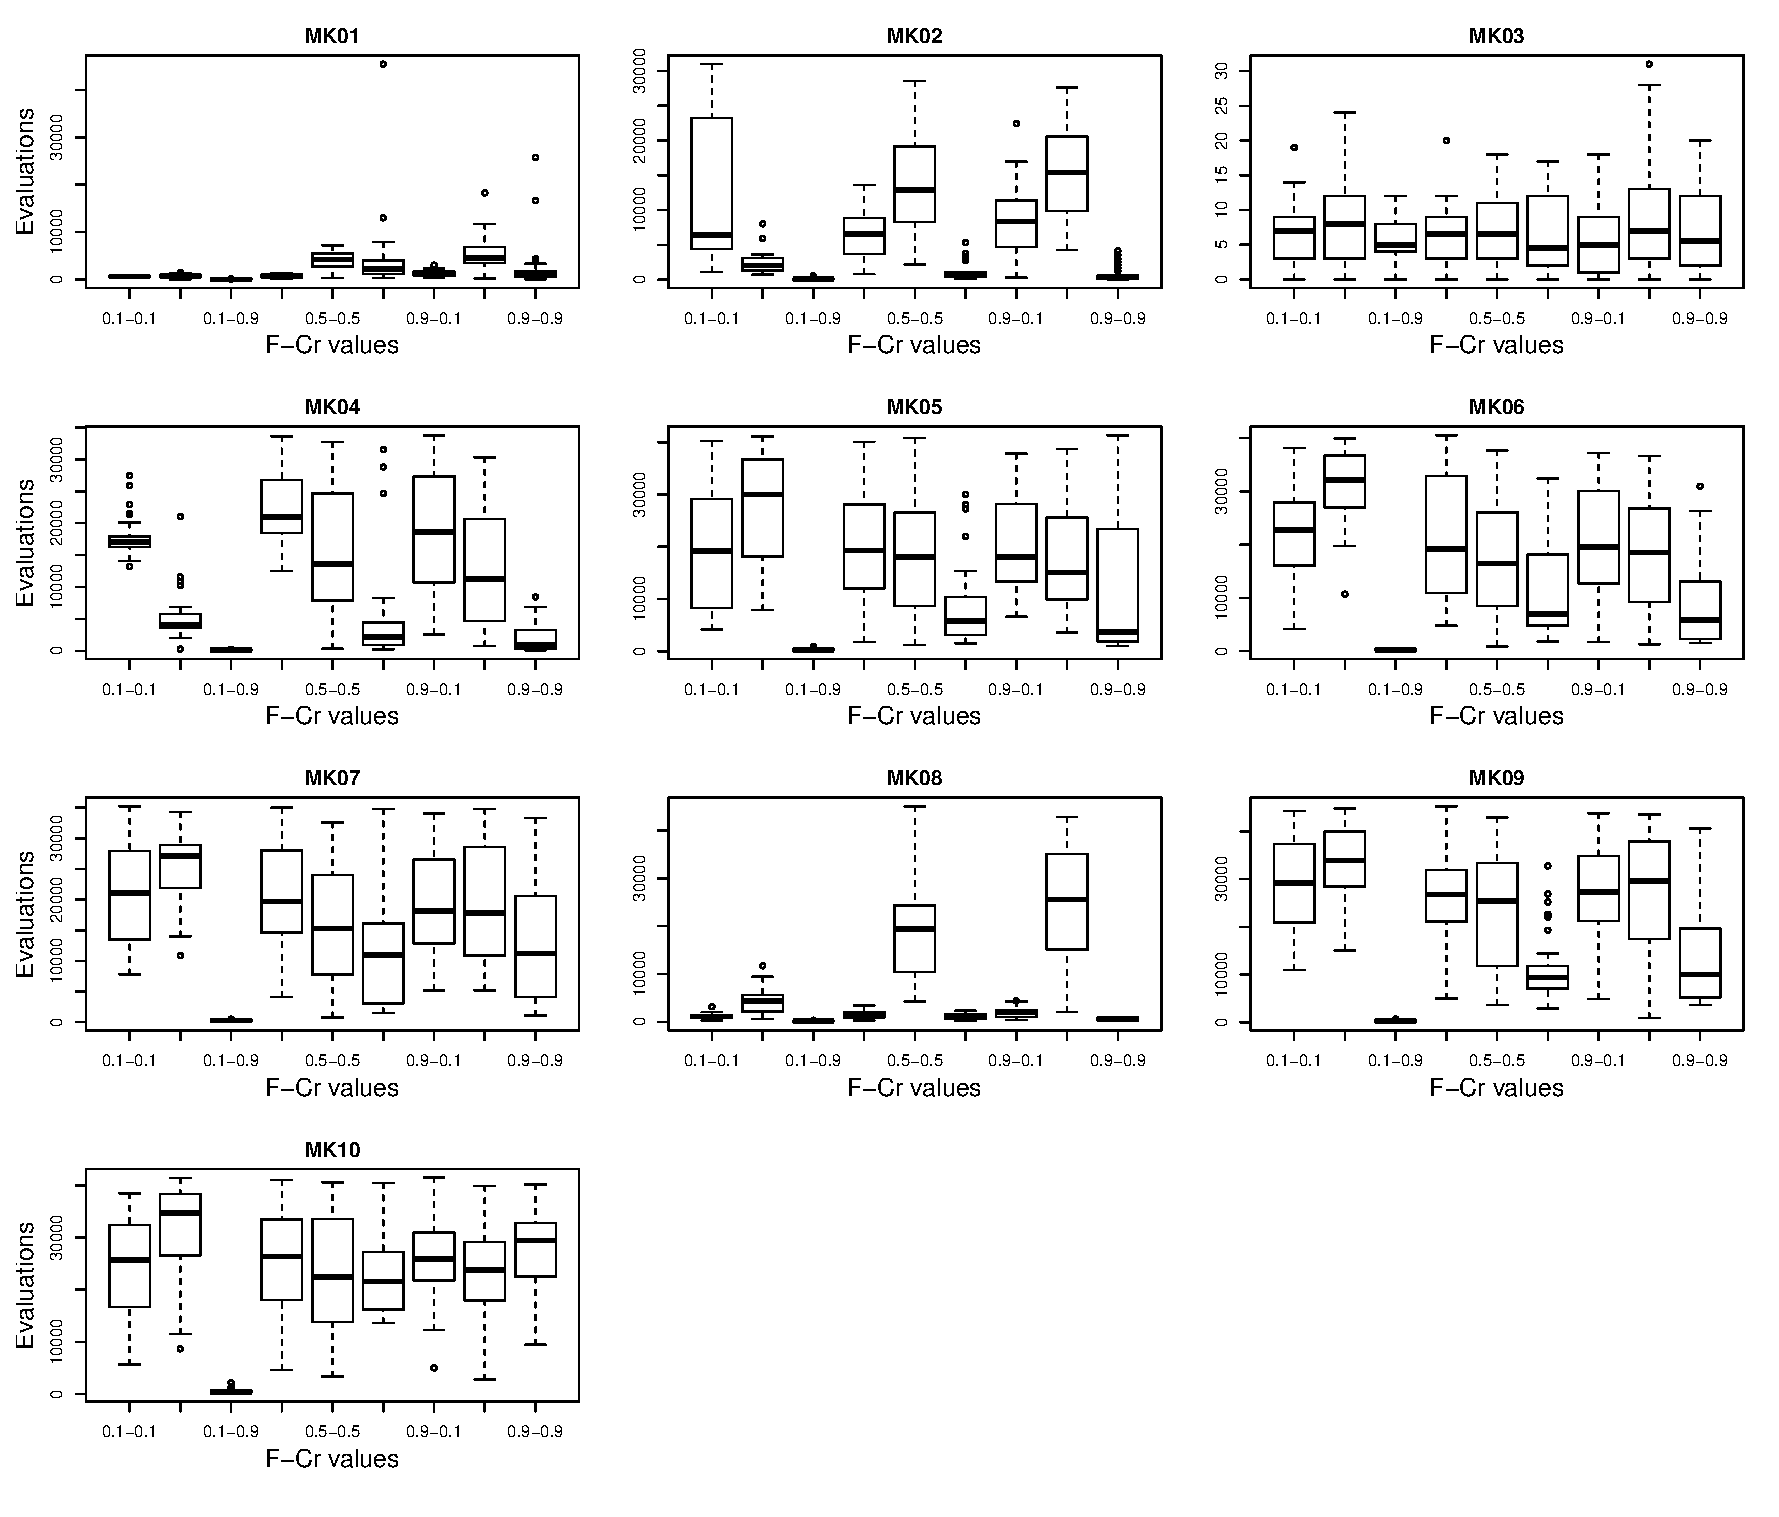
\includegraphics[width=\textwidth]{./figures/DE-evalBest.eps}
    \caption{Number of evaluations to find the best $C_{max}$ value of the DE for different combinations of $F$ and $Cr$ values considering all FJSSP instances.}
    \label{fig:DEevaluations}
    \vspace{-0.4cm}
\end{figure*}

Finally, we proceed to study the distribution of the number of evaluations to find the best $C_{max}$ value performed by DE with different combinations of different $F$ and $Cr$ values. For that purpose, Figure \ref{fig:DEevaluations} illustrates these results employing ten box plot graphs (one for each instance). In general, we observe that the DE algorithm with fewer evaluations is the one with $F\in \{0.1,0.5\}$ and $Cr=0.9$, but the combination $F=0.5$ and $Cr=0.9$ outperforms the other ones from the result quality point of view (see Table~\ref{tab:resultDE}). Consequently, we will adopt $F=0.5$ and $Cr=0.9$ as the parameter settings for the DE in the following experimentation. 

% Table generated by Excel2LaTeX from sheet 'Hoja1'
\begin{table*}[!tb]
  \centering
     \scriptsize
    \label{tab:DELS}
    \caption{Best and mean$_{\pm sd}$ $C_{max}$ values found by the DE$_{LS}$ with different values of $p_{LS}$ for all FJSSP instances.}
    \begin{tabular}{|rrcccrrr|}
    \hline
    \multicolumn{1}{|c}{} & \multicolumn{1}{|c|}{} & \multicolumn{3}{c|}{Best $C_{max}$} & \multicolumn{3}{c|}{Mean$_{\pm sd}$ $C_{max}$} \bigstrut \\
    \cline{3-8}
    \multicolumn{1}{|c|}{\textbf{Inst.}} & \multicolumn{1}{c|}{\textbf{Opt}} & \multicolumn{1}{c|}{\textbf{$p_{LS}=0.1$}} & \multicolumn{1}{c|}{\textbf{$p_{LS}=0.5$}} & \multicolumn{1}{c|}{\textbf{$p_{LS}=0.7$}} & \multicolumn{1}{c|}{\textbf{$p_{LS}=0.1$}} & \multicolumn{1}{c|}{\textbf{$p_{LS}=0.5$}} & \multicolumn{1}{c|}{\textbf{$p_{LS}=0.7$}} \bigstrut\\
    \hline
    \multicolumn{1}{|c|}{Mk01} & \multicolumn{1}{c|}{40} & \multicolumn{1}{c|}{\textbf{40}} & \multicolumn{1}{c|}{\textbf{40}} & \multicolumn{1}{c|}{\textbf{40}} & \multicolumn{1}{c|}{40.00$_{\pm 0.00}$} & \multicolumn{1}{c|}{40.00$_{\pm 0.00}$} & 40.00$_{\pm 0.00}$ \bigstrut\\
    %\hline
    \multicolumn{1}{|c|}{Mk02} & \multicolumn{1}{c|}{26} & \multicolumn{1}{c|}{27} & \multicolumn{1}{c|}{\textbf{26}} & \multicolumn{1}{c|}{\textbf{26}} & \multicolumn{1}{c|}{27.03$_{\pm 0.18}$} & \multicolumn{1}{c|}{26.96$_{\pm 0.18}$} & 26.76$_{\pm 0.43}$ \bigstrut\\
    %\hline
    \multicolumn{1}{|c|}{Mk03} & \multicolumn{1}{c|}{204} & \multicolumn{1}{c|}{\textbf{204}} & \multicolumn{1}{c|}{\textbf{204}} & \multicolumn{1}{c|}{\textbf{204}} & \multicolumn{1}{c|}{204.00$_{\pm 0.00}$} & \multicolumn{1}{c|}{204.00$_{\pm 0.00}$} & 204.00$_{\pm 0.00}$ \bigstrut\\
    %\hline
    \multicolumn{1}{|c|}{Mk04} & \multicolumn{1}{c|}{60} & \multicolumn{1}{c|}{\textbf{60}} & \multicolumn{1}{c|}{\textbf{60}} & \multicolumn{1}{c|}{\textbf{60}} & \multicolumn{1}{c|}{62.00$_{\pm 1.31}$} & \multicolumn{1}{c|}{61.30$_{\pm 0.70}$} & 61.03$_{\pm 0.66}$ \bigstrut\\
    %\hline
    \multicolumn{1}{|c|}{Mk05} & \multicolumn{1}{c|}{172} & \multicolumn{1}{c|}{173} & \multicolumn{1}{c|}{173} & \multicolumn{1}{c|}{173} & \multicolumn{1}{c|}{174.30$_{\pm 0.75}$} & \multicolumn{1}{c|}{173.00$_{\pm 0.00}$ }& 173.00$_{\pm 0.00}$ \bigstrut\\
    %\hline
    \multicolumn{1}{|c|}{Mk06} & \multicolumn{1}{c|}{58} & \multicolumn{1}{c|}{63} & \multicolumn{1}{c|}{62} & \multicolumn{1}{c|}{61} & \multicolumn{1}{c|}{64.40$_{\pm 0.56}$} & \multicolumn{1}{c|}{62.83$_{\pm 0.53}$} & 62.43$_{\pm 0.62}$ \bigstrut\\
    %\hline
    \multicolumn{1}{|c|}{Mk07} & \multicolumn{1}{c|}{139} & \multicolumn{1}{c|}{142} & \multicolumn{1}{c|}{140} & \multicolumn{1}{c|}{140} & \multicolumn{1}{c|}{143.20$_{\pm 0.69}$} & \multicolumn{1}{c|}{142.00$_{\pm 0.90}$} & 141.80$_{\pm 0.92}$ \bigstrut\\
    %\hline
    \multicolumn{1}{|c|}{Mk08} & \multicolumn{1}{c|}{523} & \multicolumn{1}{c|}{\textbf{523}} & \multicolumn{1}{c|}{\textbf{523}} & \multicolumn{1}{c|}{\textbf{523}} & \multicolumn{1}{c|}{523.00$_{\pm 0.00}$} & \multicolumn{1}{c|}{523.00$_{\pm 0.00}$} & 523.00$_{\pm 0.00}$ \bigstrut\\
    %\hline
    \multicolumn{1}{|c|}{Mk09} & \multicolumn{1}{c|}{307} & \multicolumn{1}{c|}{309} & \multicolumn{1}{c|}{\textbf{307}} & \multicolumn{1}{c|}{\textbf{307}} & \multicolumn{1}{c|}{313.10$_{\pm 2.20}$} & \multicolumn{1}{c|}{310.00$_{\pm 1.33}$} & 309.00$_{\pm 1.72}$ \bigstrut\\
    %\hline
    \multicolumn{1}{|c|}{Mk10} & \multicolumn{1}{c|}{197} & \multicolumn{1}{c|}{226} & \multicolumn{1}{c|}{225} & \multicolumn{1}{c|}{224} & \multicolumn{1}{c|}{231.10$_{\pm 2.41}$} & \multicolumn{1}{c|}{228.00$_{\pm 1.36}$} & 227.20$_{\pm 1.38}$ \bigstrut\\
    \hline
    \multicolumn{2}{c|}{}   & 4/10  & 6/10  &\multicolumn{1}{c|}{6/10}\bigstrut\\
    \cline{3-5}
    \end{tabular}%
  \label{tab:DELS}%
\end{table*}%

\subsection{Results of the DE with Local Search} \label{subsec:resDELS}

The following analysis goes into detail of what happened when the DE algorithm is enhanced with a local search procedure to solve FJSSP. The resulting algorithm is named DE$_{LS}$. For this study, we consider three different $p_{LS}$ values in the set \{0.1, 0.5, 0.7\}, i.e. we study how the frequency of the LS impacts the DE performance by using low, medium, and high probability values.

Table~\ref{tab:DELS} shows the best and the mean $C_{max}$ values, together the standard deviation, found by the DE$_{LS}$ with the different $p_{LS}$ values. The DE$_{LS}$ obtains more times the optimum when $p_{LS}=0.5$ or $p_{LS}=0.7 $.  Moreover, the KW test indicates that there are statistically significant differences among the algorithms ($p$-values are lower than the level of significance). The DE$_{LS}$ using the highest frequency ($p_{LS}=0.7$) has the lowest mean $C_{max}$ values for all instances, suggesting that the algorithm can find the optimum or near-optimal $C_{max}$ values in the majority of the runs. This assumption is reflected in the boxplot of the relative error presented in Figure \ref{fig:DELSboxplot}, which shows that the median error value is lower with the highest local search frequency.
%
\begin{figure}[!tb]
    \centering
    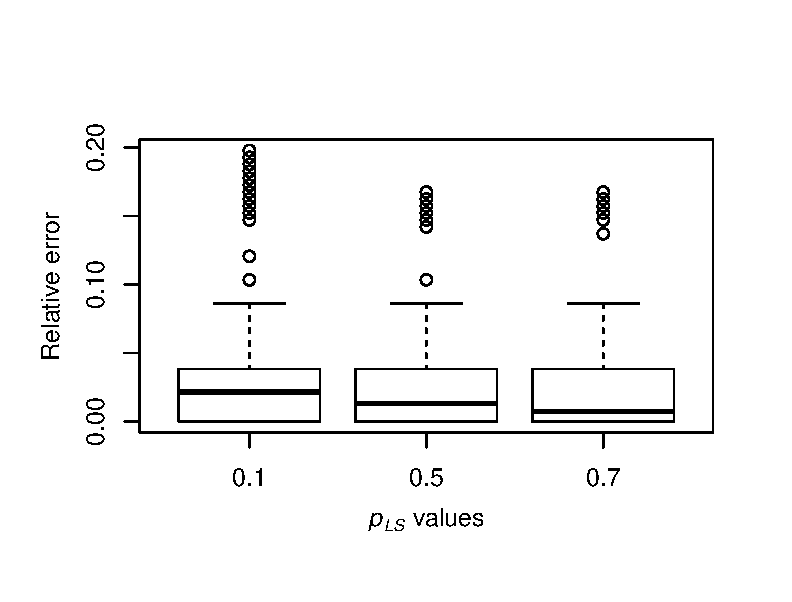
\includegraphics[width=\linewidth]{./figures/Boxplot-DELS.eps}
    \caption{Relative error of the DE$_{LS}$  for different values of $p_{LS}$.}
    \label{fig:DELSboxplot}
\end{figure}
%
\begin{figure}[!tb]
\scriptsize
\centering
   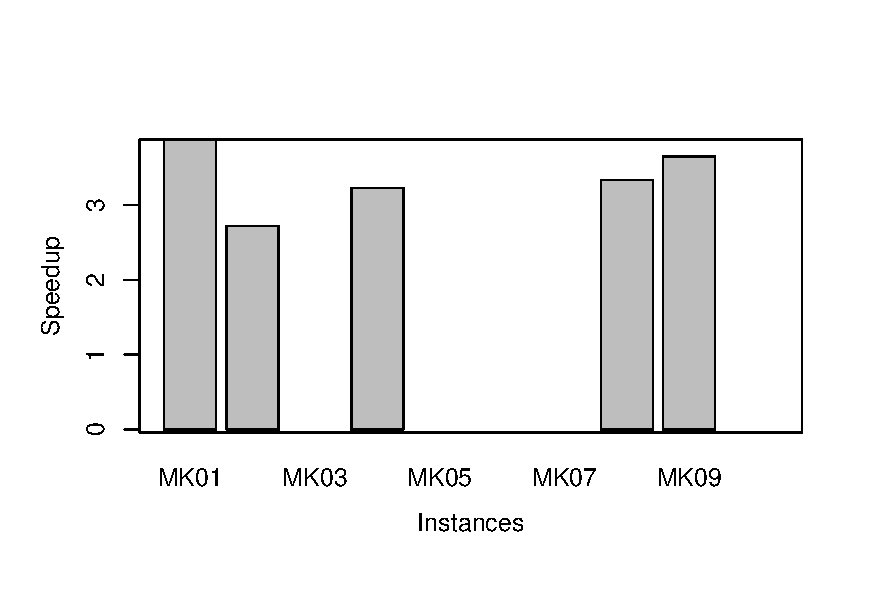
\includegraphics[width=\linewidth]{figures/speedup.eps}
   \vspace{-0.9cm}
    \caption{Speedup by FJSSP instances.}
    \label{fig:speedup}
\end{figure}
%
\begin{table*}[!tb]
\scriptsize
  \centering
  \caption{Comparison between DE$_{LS}$ and population-based metaheuristics from the literature}
    \begin{tabular}{|l|cccccccccc|}
    \hline
    \multicolumn{1}{|r}{} & \multicolumn{1}{l}{MK01} & \multicolumn{1}{l}{MK02} & \multicolumn{1}{l}{MK03} & \multicolumn{1}{l}{MK04} & \multicolumn{1}{l}{MK05} & \multicolumn{1}{l}{MK06} & \multicolumn{1}{l}{MK07} & \multicolumn{1}{l}{MK08} & \multicolumn{1}{l}{MK09} & \multicolumn{1}{l|}{MK10} \\
    \hline
    DE$_{LS}$   & \textbf{40} & \textbf{26} & \textbf{204} & \textbf{60} & 173   & 61    & 140   & \textbf{523} & \textbf{307} & 224 \\
    hGA   & \textbf{40} & \textbf{26} & \textbf{204} & 62    & \textbf{172} & 65    & 140   & \textbf{523} & 310   & 214 \\
    BEDA  & \textbf{40} & \textbf{26} & \textbf{204} & \textbf{60} & \textbf{172} & 60    & \textbf{139} & \textbf{523} & \textbf{307} & 206 \\
    IACO  & \textbf{40} & \textbf{26} & \textbf{204} & \textbf{60} & 173   & 60    & 140   & \textbf{523} & \textbf{307} & 208 \\
    HDE   & \textbf{40} & \textbf{26} & \textbf{204} & \textbf{60} & \textbf{172} & \textbf{57} & \textbf{139} & \textbf{523} & \textbf{307} & \textbf{198} \\
\hline
    \end{tabular}%
  \label{tab:comparison}%
\end{table*}%
%
Now, to determine if the DE$_{LS}$ can improve the $C_{max}$ values found by the DE, we perform a comparison of relative error values shown in Figure~\ref{fig:DEboxplot} and the ones from Figure~\ref{fig:DELSboxplot}. We can observe that the DE$_{LS}$ algorithm with $p_{LS}=0.7$ obtains lower relative errors than those presented by DE, which indicates the advantage of incorporating local search into the DE framework.

\subsection{Results of the DE$_{LS}$ and Parallelism} \label{subsec:resparallelDELS}

In this section, we study the behavior of the parallel DE described in Section~\ref{subsec:parallelHDE}. The most important measure of a parallel algorithm is speedup. This measure is defined as the ratio of the sequential execution time (DE$_{LS}$ execution time, in this case) to the parallel execution time. For this analysis, we consider the weak speedup~\cite{albaMeta2005}. For that reason and following the best practice by Luque and Alba~\cite{Luque:2013:PGA:2564896}, the stopping criterion is based on the quality of the final solution achieved by the algorithms, which is set to the optimum for each FJSSP instance (see column Opt. of Table~\ref{tab:resultDE}). Consequently, the speedup values are only reported for those instances for which the DE$_{LS}$ algorithm obtains the optimum value.

Once we established the execution times of the DE$_{LS}$ and the parallel DE$_{LS}$, we calculate the speedup values. Figure~\ref{fig:speedup} shows that the use of parallelization is worthwhile, as we expected. The parallel DE$_{LS}$ allows to reduce the search time and obtains a very good speed up, nearby linear (the ideal speedup value is 4, the number of available cores per machine).

\section{Comparison of DE$_{LS}$ with the Literature} \label{sec:compara}

Finally, we present a comparative assessment of the $C_{max}$ values obtained by the DE$_{LS}$ with the ones of several competitive algorithms present in the literature to solve FJSSP. This allows us to determine the goodness of the metaheuristics considered in this work. In this comparison different population-based metaheuristics to solve FJSSP are considered: 
\begin{enumerate}[label=\textit{\roman*})]

\item hGA~\cite{tang2011}: a hybrid algorithm combining chaos particle swarm optimization with genetic algorithm

\item BEDA~\cite{Wang2012917}: a bi-population based estimation of distribution algorithm

\item IACO~\cite{WANG2017}: an ant colony optimization

\item HDE~\cite{YUAN2013246}: a hybrid differential evolutionary algorithm 

\end{enumerate}

Table~\ref{tab:comparison} shows that the $C_{max}$ values obtained by DE$_{LS}$ are similar to the ones of remaining algorithms, for the majority of the ten instances. This observation suggests that the DE$_{LS}$ proposed in this work is a competitive algorithm to solve FJSSP. Comparisons regarding computational effort are hard to be carried out because the majority of the works do not report the number of evaluations. Consequently, the relative efficiency of referred algorithms is difficult to contrast to obtain meaningful comparisons.




\section{Conclusions} \label{sec:conclu}

This paper presented a simple DE algorithm to solve FJSSP, which has significant application value in modern manufacturing environments. In this study, we considered a real-valued representation to code a valid schedule for FJSSP. Consequently, we maintained the good properties of the DE as a problem optimizer because it still works on the continuous domain. The DE was enhanced with a very simple local search procedure (DE$_{LS}$) to balance the exploration and exploitation of the search space. Furthermore, each iteration of the DE$_{LS}$ was parallelized to speed up the computation using the global parallelization model. 

Computational results indicated that the DE with a combination of medium $F$ and high $Cr$ values obtained good quality of $C_{max}$ values in a less number of evaluations. Moreover, the DE$_{LS}$ with a high probability of application of the local search procedure was able to improve the best solutions found by the DE for FJSSP in a major number of instances. We also obtained a decrease in execution times by introducing parallelization to the DE framework without changing the algorithm behavior. Finally, the comparison of our proposal with several algorithms in the literature indicated that we develop a competitive approach. As a consequence, our simple DE proposal is an efficient and competitive optimizer for this NP-hard problem.

As future research activities, we will plan to extend the study by including another set of instances with high dimensionality. Furthermore, FJSSP variants with more constraints will be evaluated considering the approaches developed in this article.


\begin{small}

\competinginterests{
The authors have declared that no competing interests exist.
}

\funding{
The authors acknowledge the support of Universidad Nacional de La Pampa, Universidad Nacional de Río Cuarto, and the Incentive Program from MINCyT. The second author is also funded by CONICET. 
}

\authorcontributions{
%This paragraph is required and authors must declare their contribution here. Guidance and criteria for authorship can be found in the section "Publication Ethics and Malpractice Statement" of our website.
% Please use initials to refer to each author's contribution in this section, for example: "
All authors conceived the idea, wrote the program, conducted the experiments, analyzed the results, and finally, wrote and revised the manuscript. Moreover, all authors read and approved the final manuscript.
}

%\acknowledgements{
%This paragraph is optional and is meant for acknowledgements information.
%}

\bibliographystyle{IEEEtran}
\bibliography{biblioFJSSP}


\end{small}

\vspace*{2cm}


\cornersize{.2} 
\setlength{\fboxsep}{8pt}

\ovalbox {

\begin{minipage}{7cm}
\textbf{Citation:} F. Morero, C. Bermudez, C. Salto, 

\emph{Parallelism and Hybridization in Differential Evolution to solve the Flexible Job Shop Scheduling Problem}. Journal of Computer Science \& Technology, vol. 20, no. 1, pp. X-X, 2020.

\textbf{DOI:} XXX

\textbf{Received:} March 18,2020
\textbf{Accepted:} %August 15, 2017.

\textbf{Copyright:} This article is distributed under the terms of the Creative Commons License CC-BY-NC.
\end{minipage}
}




\end{document}
